% !TeX root = ../thuthesis-example.tex

\chapter{高效算子设计}
\thusetup{
  cite-style = super,
}

\section{灵活规约定义}\label{sec:flexible-reduciton}
规约是稀疏稠密混合张量代数的核心操作。规约的数学定义如式\eqref{eq:reduction}。其中$x \in X$,每个$x$有两个参数,一个是$id\in ID$,另一个是$val$。其中$id$是可以哈希的键值,$val$是可以被运算符$\oplus$运算的值。
$X$是由$x$组成的列表,$Out$是输出列表,由$ID$索引。

\begin{equation}
  Out[i] = \oplus_{x\in X;x.id=i} x.val
  \label{eq:reduction}
\end{equation}
\begin{figure}[h]%
  \centering
  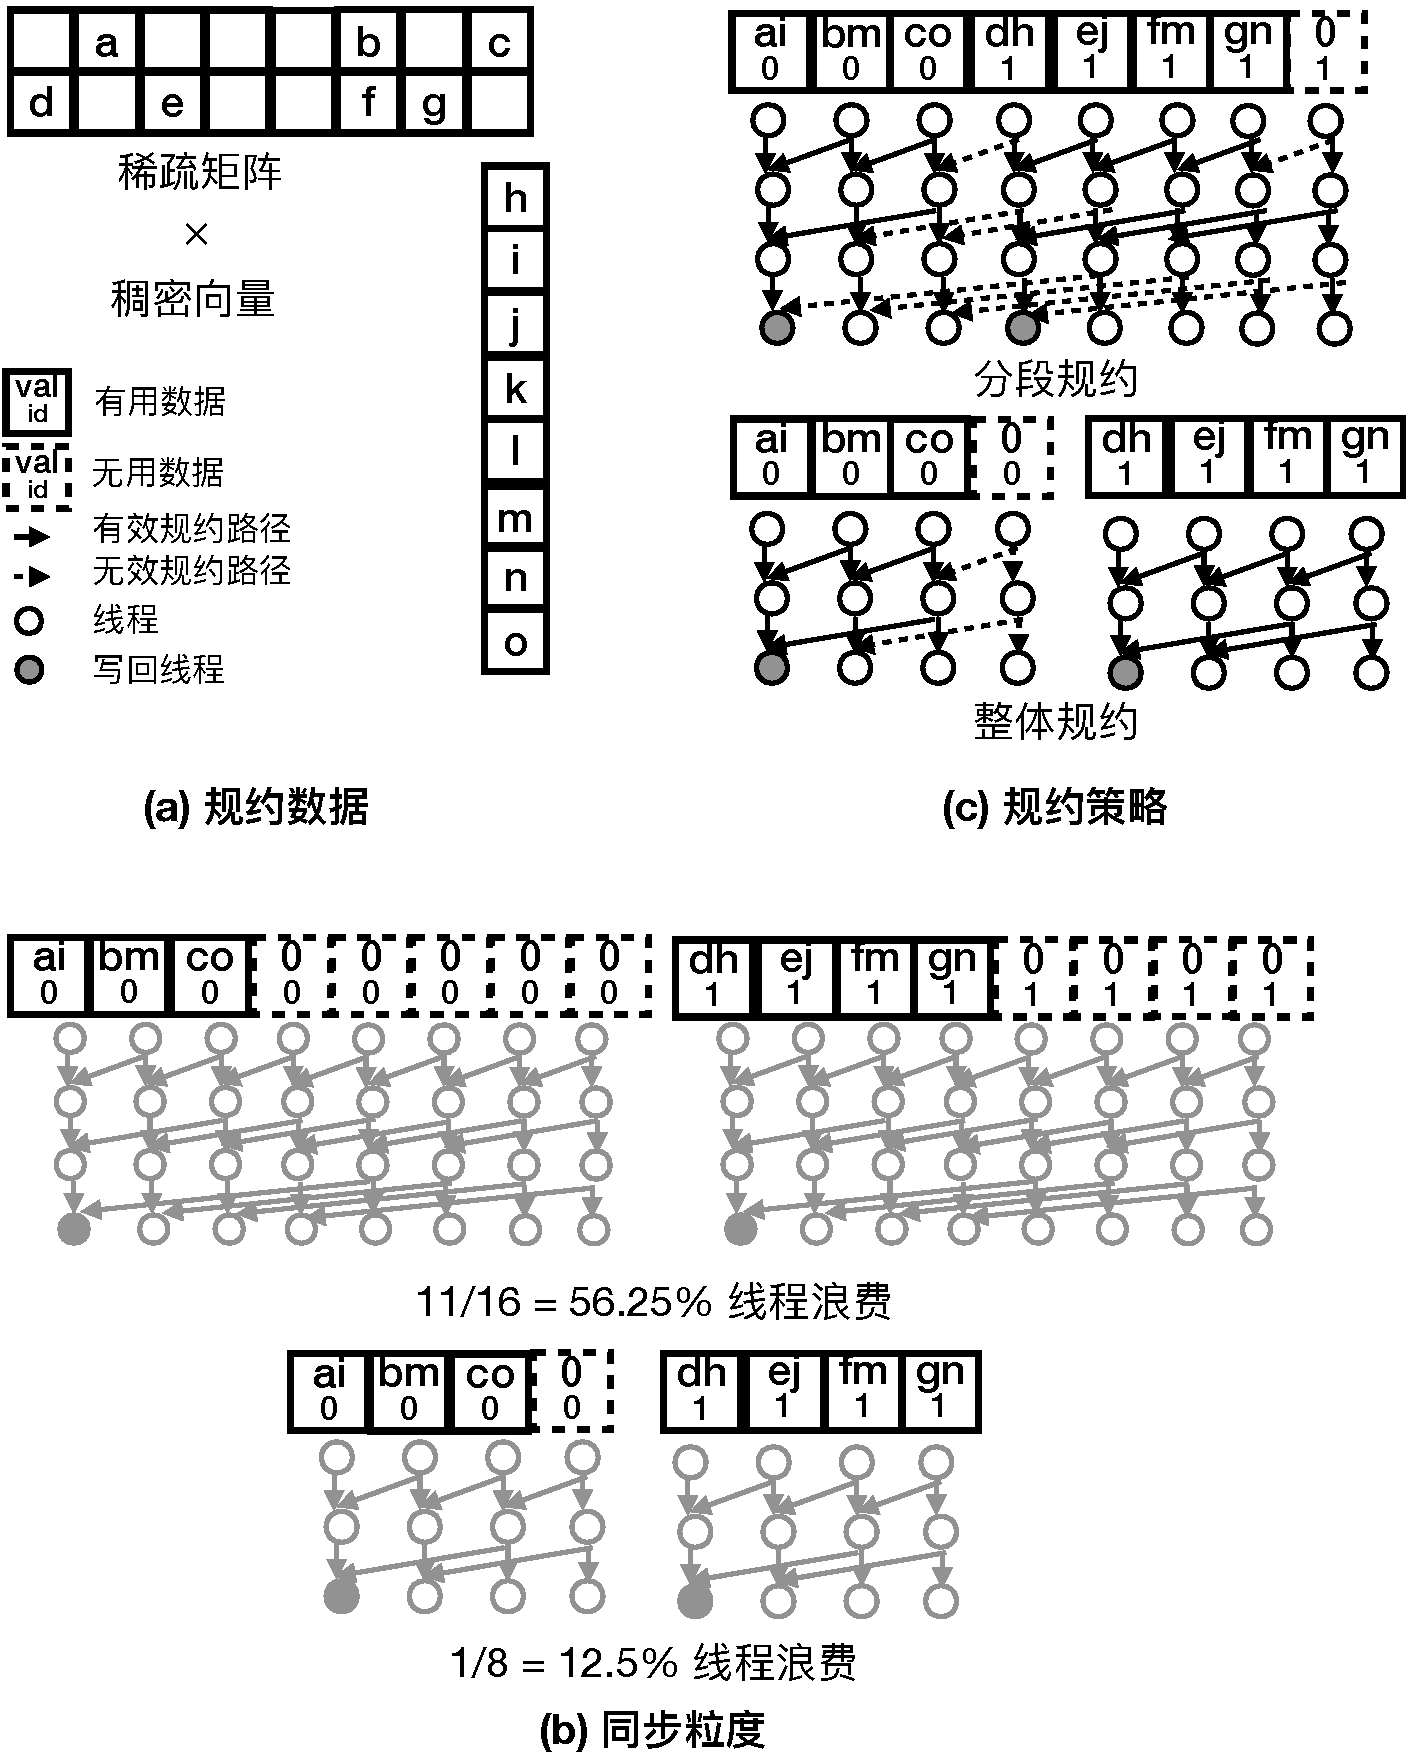
\includegraphics[width=0.5\textwidth]{reduction.pdf}
  \caption{不同规约粒度和规约方法示意图}
  \caption*{(a)被规约的数据。其中有一个行数为2列数为8的稀疏矩阵和一个长度为8的稠密向量做矩阵向量乘法。(b)不合适的规约粒度会导致线程浪费,该子图中未区分有效和无效规约路径。(c)分段规约和整体规约。在这个例子中分段规约有2个写回线程。整体规约始终只有1个写回线程。}
  \label{fig:reductions}
\end{figure}
同时,不同的规约粒度也可能影响线程利用率,进一步影响算子性能。PRedS\cite{yu2021exploiting}虽然研究了并行规约粒度对性能的影响,但是它只局限于$X$中所有元素的$id$相等的情况,即稠密规约。本文更进一步,研究稀疏规约,即$X$中元素的$id$不相等的情况。
因为$id$不相等,所以不是所有元素都要累加到同一个输出上。因此,本文引入了有用数据,无用数据,有效规约路径,无效规约路径,和写回线程等概念。
这些概念的产生与GPU的线程同步策略密切相关。GPU会同步一组线程,而这组线程的线程数是2的次方且不大于32。这组线程的线程数我们称之为同步粒度。线程可以向同一线程组的另一的线程种传递本线程持有的寄存器数据。有用数据的意思是对最后结果起作用的数据,即$X$中的元素。无用数据是规约粒度和待规约元素个数不匹配引入的数据。在图~\ref{fig:reductions}(b)的两个例子中,均采用整体规约。
因为整体规约要求所有被规约元素的$id$相同,所以当规约粒度超过$id$相同的元素数目时,就需要补充一些$val$是$\oplus$运算意义下的零元(在实数加法中就是0)的元素。这些元素只是起到占位作用,其$val$并没有加到输出结果中,因此被称为无用数据。
相应地,有效规约路径表示该路径连接的两种线程中,起始线程的值会最终叠加到写回线程的值中。无效规约路径则是为了避免GPU各线程执行路径不一致问题而引入的执行路径。
GPU提供了多种规约方式,写回线程表示该线程的寄存器中存放着最终写入$Out$的数据。分段规约表示一个线程组规约给定数目的$X$中的元素,整体规约表示一个线程组规约$X$中给定$id$的元素。分段规约根据该线程组处理的不同$id$数量可以有多个写回线程,整体规约因此$id$相同,所以只有1个写回线程。多个写回线程的线程号取决于$X$中的$id$分布,因此在运行时决定。两种规约的示意图如图~\ref{fig:reductions}(c)所示。
不同的输入数据适合不同的规约,比如在DA-SpMM\cite{dai2022heuristic}的对比实验中,分段规约和整体规约在不同数据集上的性能相比既可能好,也可能差2到4倍。

\section{灵活规约优化空间扩展}
\subsection{硬件模型}\label{sec:hwmodel}
因为规约是稀疏稠密混合张量代数的核心操作,所以优化空间扩展核心是多少数据需要被规约以及采用何种规约策略。本文将逻辑上原子的计算单元设置为线程。一个线程可以一个串行程序。所有线程独立执行相同的程序。每个线程有各自的输入数据,同时根据threadId区分。
线程可以成组做同步规约,规约并行度(粒度)可以是2,4,8,16或32.我们将GPU的计算建模为逻辑上无限多的平行线程,同时定义GPU可以提供的线程数为源并行度。在这个模型中我们没有考虑共享内存、线程块层级以及线程到流式处理器的映射策略等。本文把这些视作在基础并行模式确定后合理的部署细节。换句话说,在本文基于灵活规约扩展后的优化空间中,每一种优化策略对应许多不同的部署技术。这样扩展后的优化空间可以为GPU细节优化提供更简洁的视角。
\subsection{原子并行}\label{sec:atomicparallel}
为了具体定义并行模式,本文提出了原子并行概念。处于原子并行状态的一个程序不能继续被并行。换句话说,原子并行规定了一个线程执行的数据量。正式地,本文定义原子并行是最小数据的笛卡尔积。最小数据数据是一个线程所能处理的最小某类数据量。原子并行可以用来构建在GPU上执行的稀疏稠密混合代数的优化空间。
当然分块技术、精细管理共享内存、线程映射等优化技术对于GPU上的稀疏稠密混合代数也很重要\cite{hidayetouglu2020scale,mehrabi2021learning,xin2021fast,gale2020sparse}。这些技术对于稠密张量相对稀疏张量形状较大时更有利,比如在SpMM中稠密矩阵列数大于128时。因为计算的负载会很重,想稠密矩阵的向量化数据读取会成为瓶颈。
当稠密张量相对于稀疏张量形状较小,比如SpMM中稠密矩阵列数小于8时,每个线程的工作负载都较小,此时吞吐率被最长的线程组执行时钟数限制,因此需要更好的工作负载均衡。

下面以SpMM为例展示利用原子并行构建灵活规约优化空间扩展的步骤。SpMM有两种正交的原子并行:最小数据可以是$\{\frac{1}{g},1,g\}$个稀疏矩阵的非零元和$\{\frac{1}{c},1,c\}$个稠密矩阵列;也可以是$\{\frac{1}{g},1,g\}$个稀疏矩阵行和$\{\frac{1}{c},1,c\}$个稠密矩阵列。
其中$c\in \mathbb{Z^+}$和$g\in \mathbb{Z^+}$是可以调优的参数。尽管他们都可以是1但是他们和1的意义不同,因为他们是可以调优的。因此基于原子并行的SpMM灵活规约粒度优化空间扩展可以用$<x\,nnz , y\,col>$或者$<x\,row, y\,col>$描述。
源并行度只会向原子并行度中的一个元素做乘法。例如,给定源并行度$r$,针对第一种原子并行线程执行的数据量可以定义为$<r \times x\,nnz , y\,col>$或者$<x\,nnz, r \times y\,col>$;针对第二种原子并行线程执行的数据量可以定义为$<r \times x\,row , y\,col>$或者$<x\,row, r \times y\,col>$。
除此以外,分数类型的数据意味着不同线程会在同样的单个数据上执行。比如$<\frac{1}{g}\, row, 1\, col>$表示$g$个线程合作在同一行上执行。
\subsection{空间定义}\label{sec:spacedef}
依然使用SpMM的例子,我们用原子并行和规约并行 $\{<...>,r\}$ 来定义一个SpMM算子。$<...>\in \{\frac{1}{g},1,g\}\, nnz \times \{\frac{1}{c},1,c\}\, col $ or $\{\frac{1}{g},1,g\}\,row \times \{\frac{1}{c},1,c\}\,col$。他们描述了最小数据。同时规约并行度$r\in\{2,4,8,16,32\}$指定了每次有多少线程同步。 
图~\ref{fig:space3d}展示了SpMM的优化空间。但是,基于原子并行和规约并行构建的优化空间中不是所有点都合法。图~\ref{fig:space}中展示了空间剪枝的细节。优化空间中合法的点有3个条件:
\begin{enumerate}
  \item $\{<\frac{1}{g}\,nnz , x\,col>,r\}$, $\{<x\,nnz , \frac{1}{c}\,col>,r\}$ 
  是非法的,因为一个非零元一定与稠密矩阵中的一个点相乘。
  \item $\{<\frac{1}{g}\,row, x\,col>,r\}(\frac{r}{g}<1)$
  是非法的,因为整体规约只能有一个写回线程。
  \item $\{<\frac{1}{g}\,row , \frac{1}{c}\,col>,r\}$
  是非法的,因为它和源并行只能与原子并行中的一个元素相乘矛盾
\end{enumerate}
\begin{figure}[h]%
  \centering
  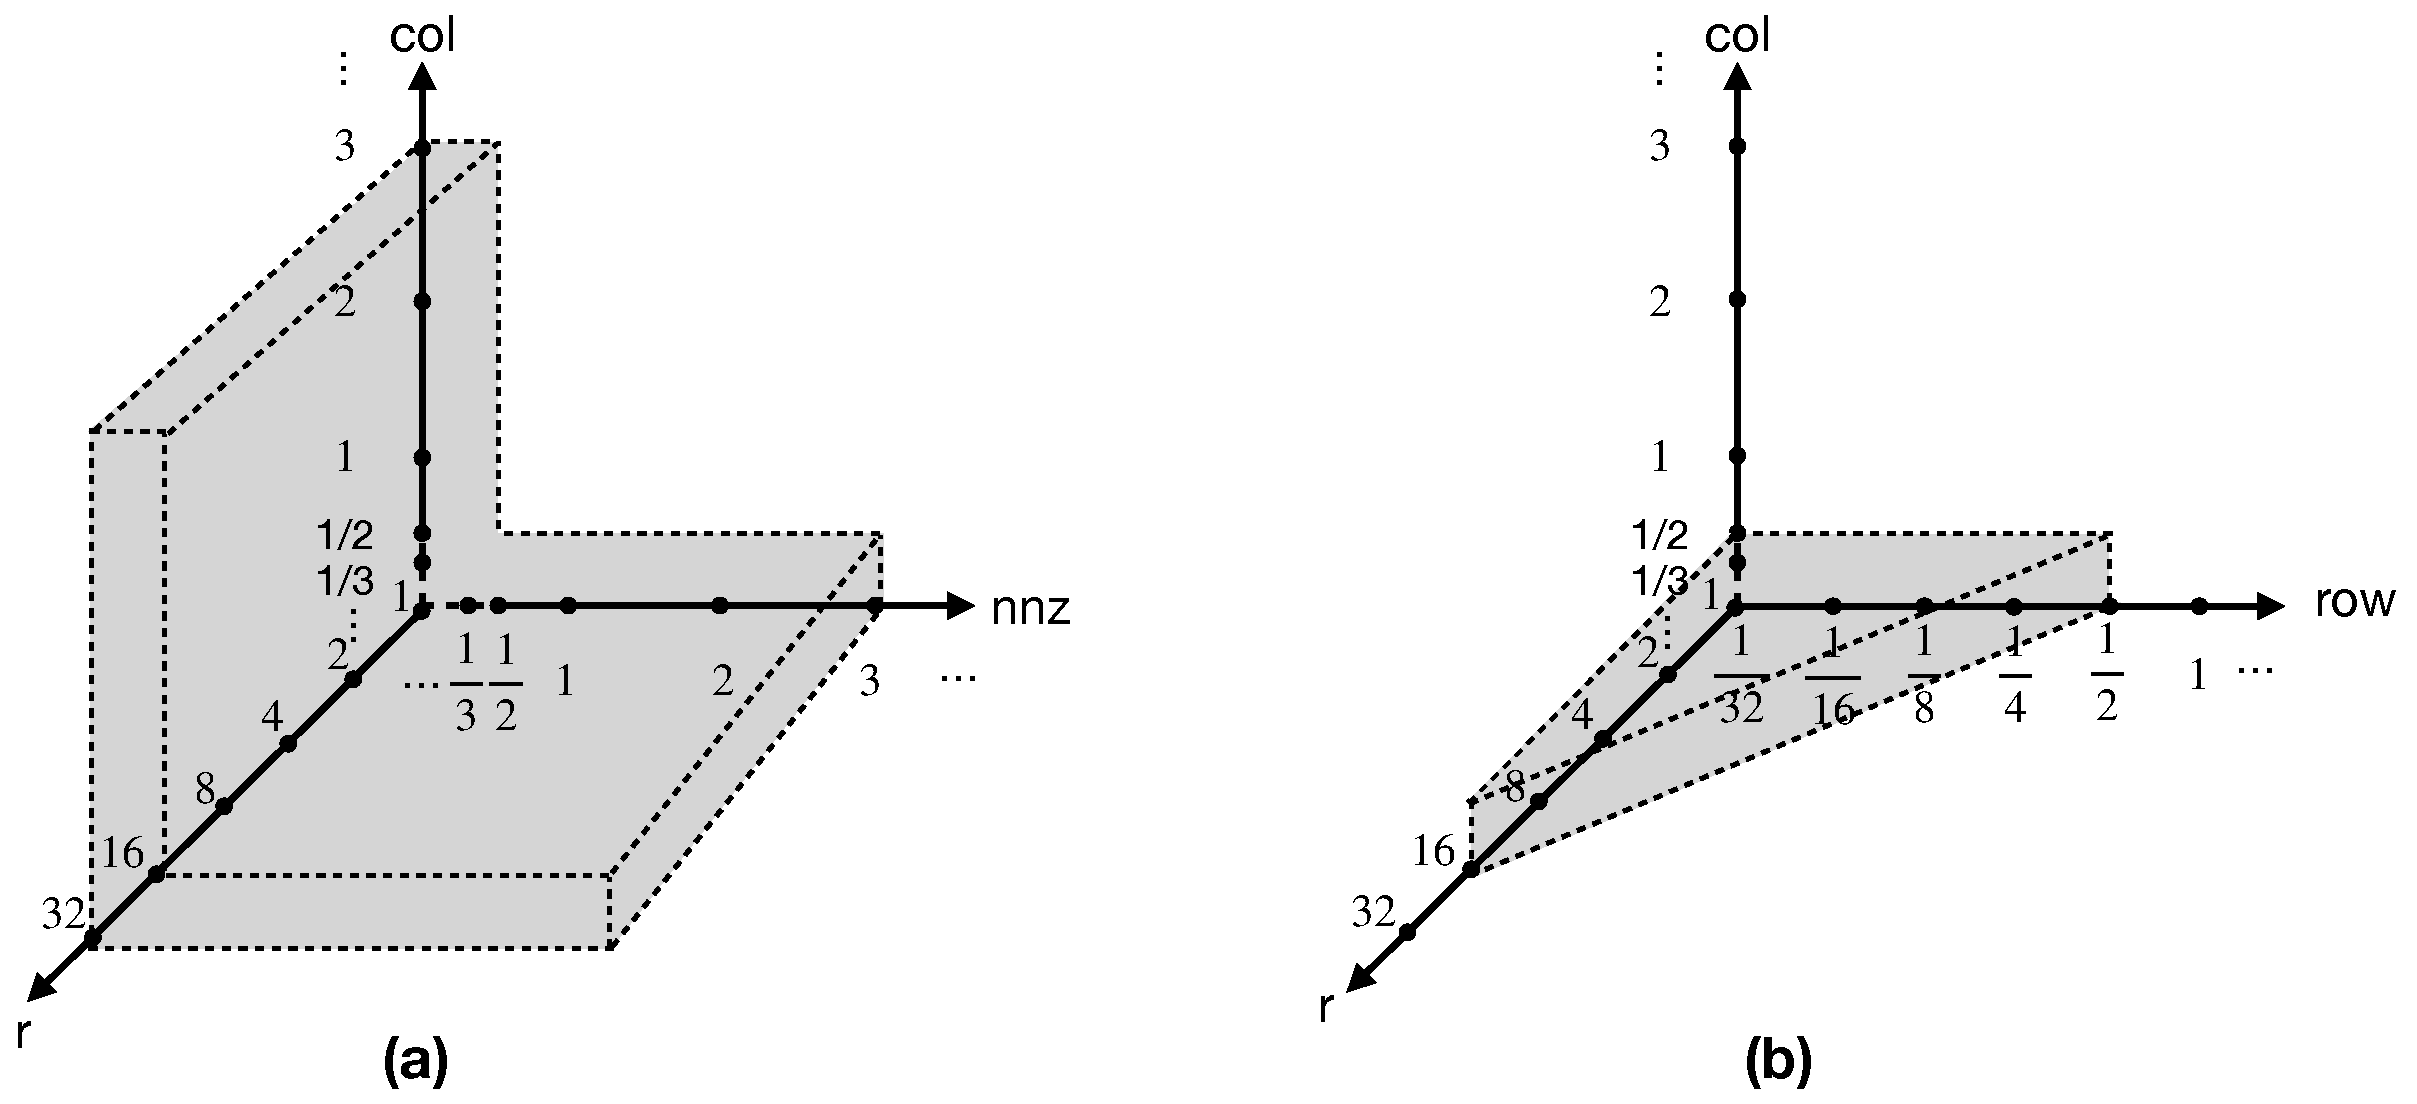
\includegraphics[width=0.9\textwidth]{space_3d.pdf}
  \caption{SpMM灵活规约优化空间扩展示意图}
  \caption*{灰色区域是非法区域,在每个坐标轴根部的虚线部分代表结束点和硬件相关。}
  \label{fig:space3d}
\end{figure}
\begin{figure}[h]%
  \centering
  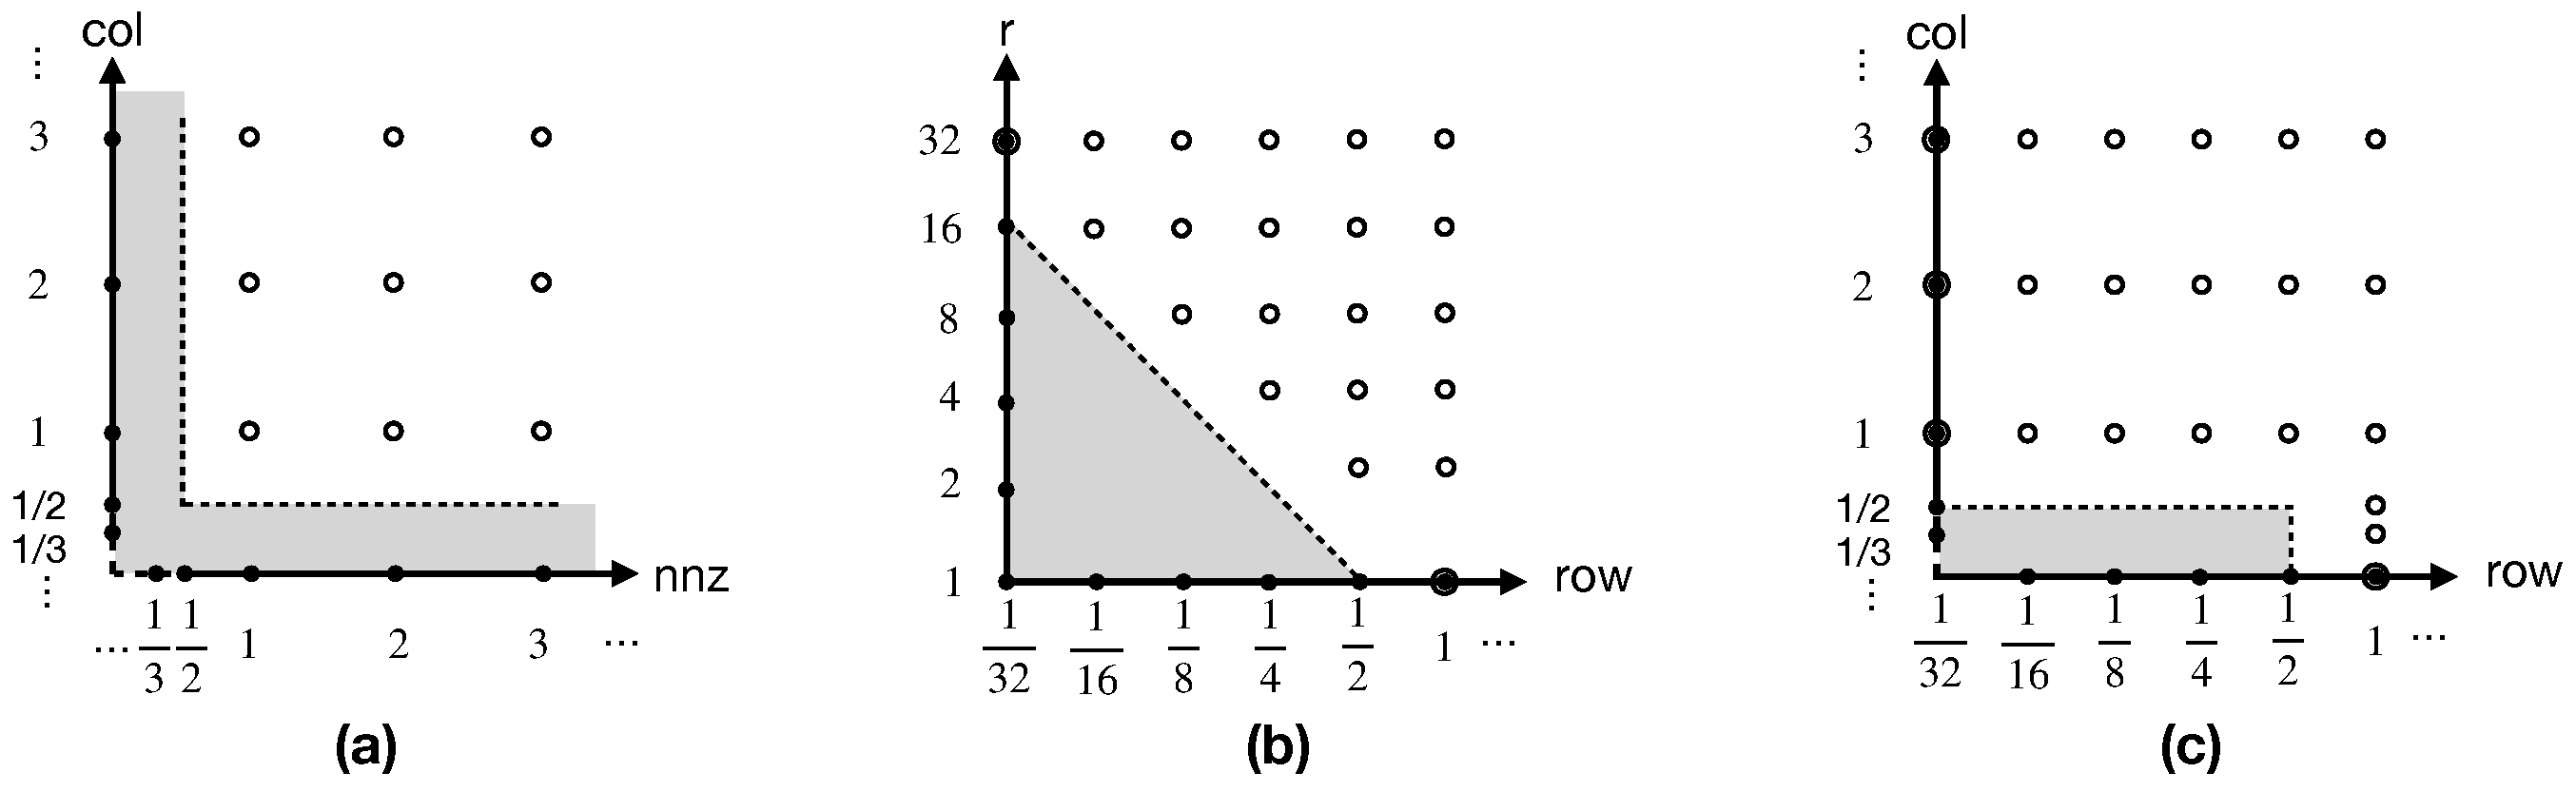
\includegraphics[width=0.9\textwidth]{space.pdf}
  \caption{SpMM灵活规约扩展优化空间的二维投影示意图}
  \caption*{灰色区域是非法的,空心圈是合法的点。子图(a),(b),(c)分别对应规则1,2,,3。}
  \label{fig:space}
\end{figure}
\begin{figure}[h]%
  \centering
  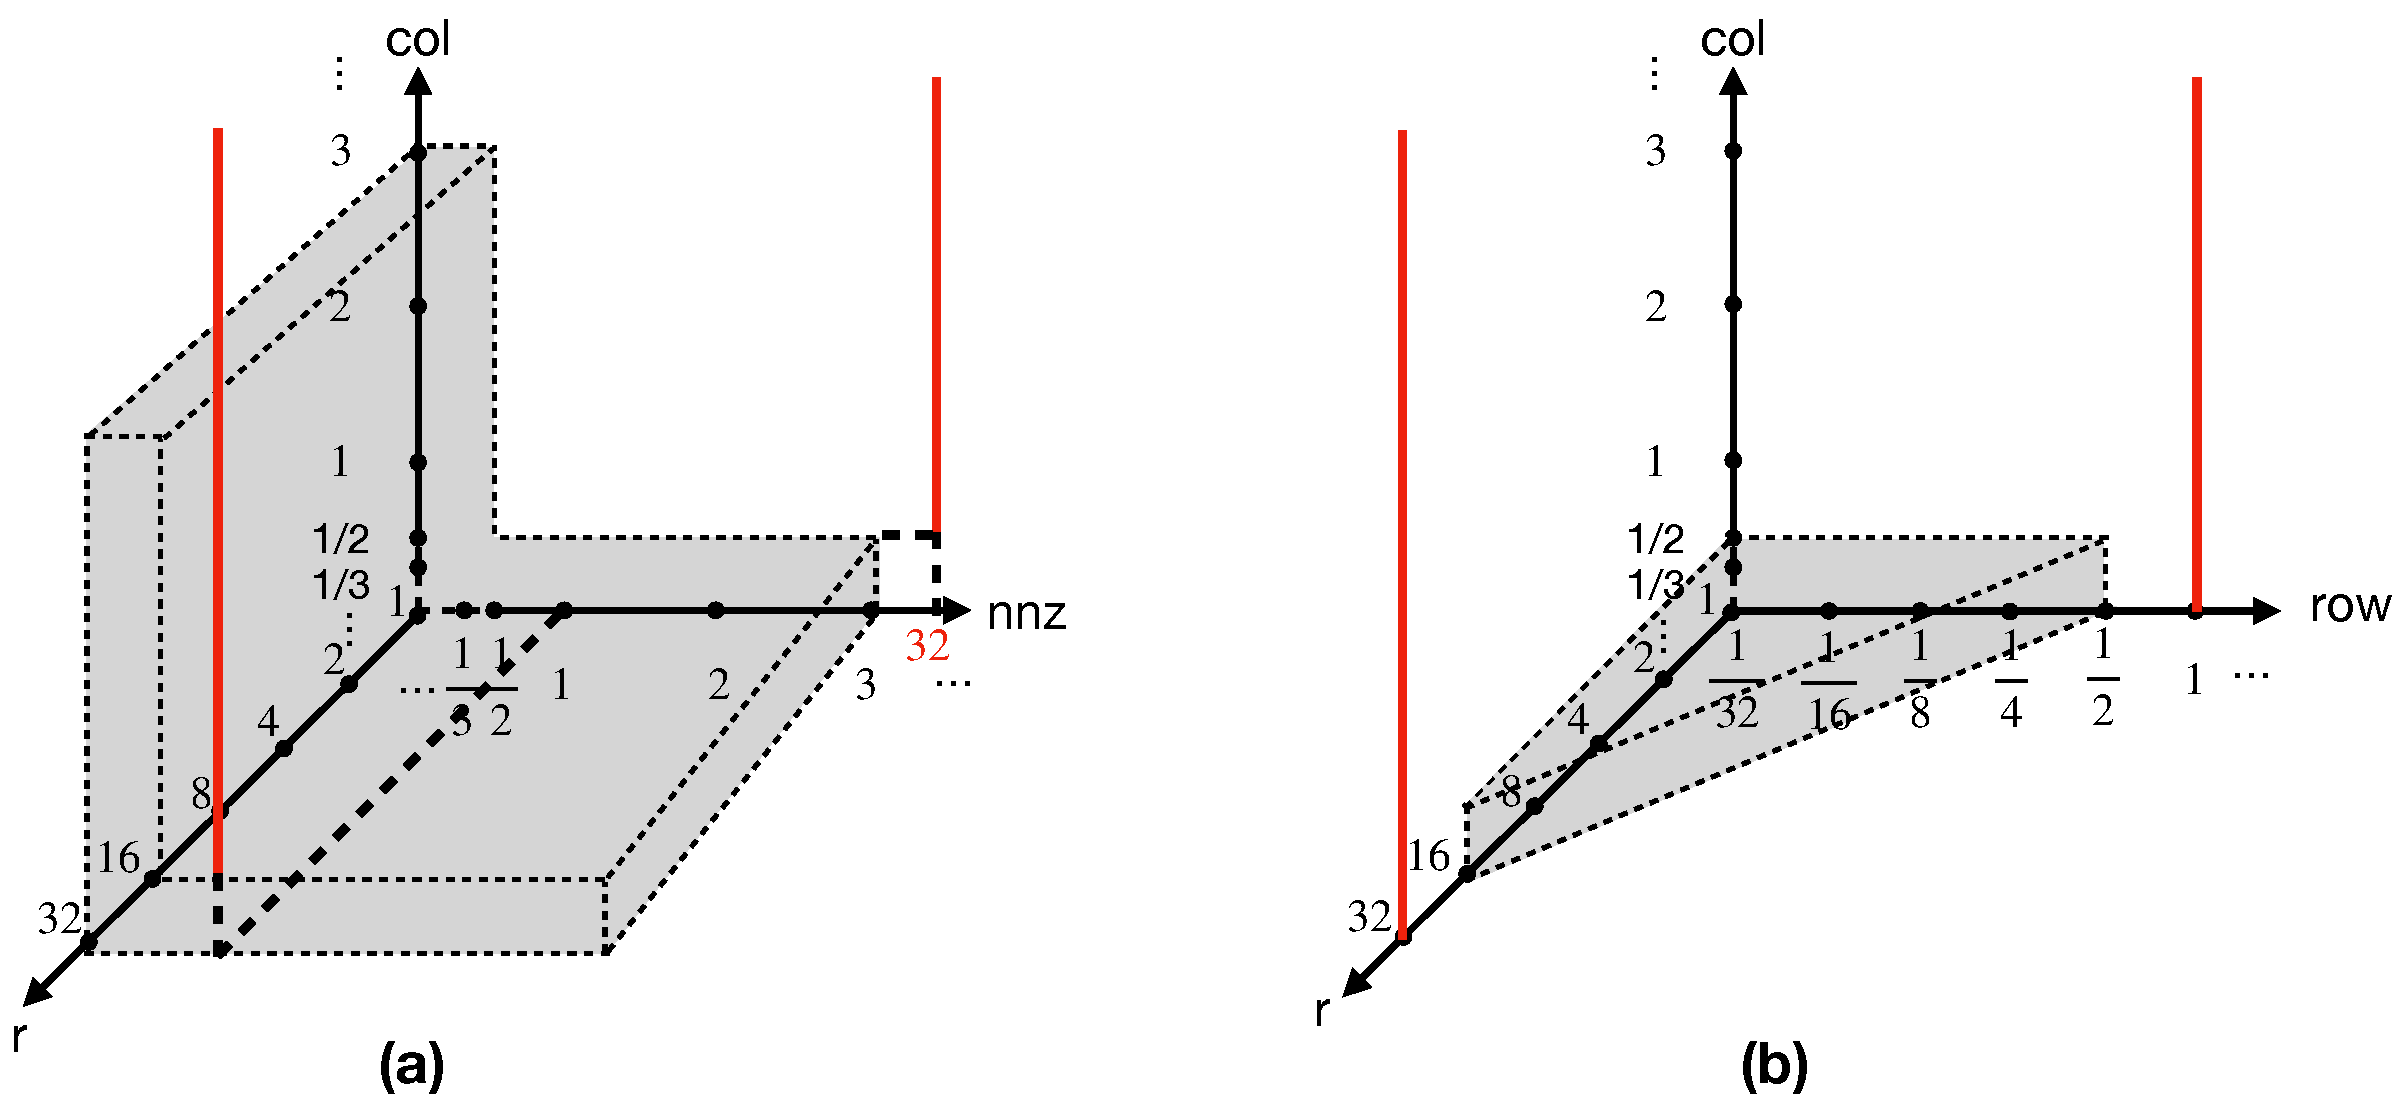
\includegraphics[width=0.9\textwidth]{daspmm.pdf}
  \caption{DA-SpMM的四种算法在灵活规约优化空间扩展中的位置}
  \caption*{红色代表DA-SpMM包含的优化空间,灰色区域是非法区域,在每个坐标轴根部的虚线部分代表结束点和硬件相关。}
  \label{fig:daspmm}
\end{figure}
最新的SpMM算子库设计空间DA-SpMM包含在上面基于原子并行构建的灵活规约优化空间扩展中。DA-SpMM提出了一个三维的SpMM算法设计空间,分别有三个维度:行/非零元均衡、行/列起始循环,并行/串行规约,论文中分别简称RB/EB、RM/CM、PR/SR。
因为行/列起始循环不影响并行策略,所以我们只考虑EB+PR,RB+PR,EB+SR,RB+SR四种算法。如图~\ref{fig:daspmm}所示,在灵活规约优化空间扩展中EB+PR是$\{<1\,nnz , c\,col>,32\}$,RB+PR是$\{<\frac{1}{32}\,row, c\,col>,32\}$,EB+SR是$\{<32\,nnz,c\,col >,1\}$,
RB+SR是$\{<1\,row,c\,col >,1\}$。其中$c$对应DA-SpMM中的向量化参数,$g$表示灵活规约中的线程组大小。尽管在真实GPU中由于源并行度有限,导致$1\,row$或$1\,nnz$可能会有超过1行或1个非零元的最小数据。但是我们仍然将这类算法归类为空间中的$1\,row$或$1\,nnz$点。


\section{实验结果}
\subsection{实验环境}\label{sec:exp-env}
本节在Turing(图灵),Volta(伏打)和Ampere(安培)三代GPU架构上进行算子性能测试,该三种架构分别对应RTX 2080,Tesla V100和RTX 3090:
\begin{itemize}
\item NVIDIA RTX 3090. Compute Capability 8.6 (68 Ampere SMs at 1.395 GHz, 24 GB GDDR6x, 936 GB/s bandwidth).
\item NVIDIA RTX 2080. Compute Capability 7.5 (46 Turing SMs at
1.515 GHz, 8 GB GDDR6, 448 GB/s bandwidth).
\item NVIDIA Tesla V100. Compute Capability 7.0 (80 Volta SMs at
1.370 GHz, 16 GB HBM2, 900 GB/s bandwidth). 
\end{itemize}
同时使用11.6版本的NVCC和11.6版本的CUDA,并采用和DA-SpMM相同的编译选项。我们用英伟达官方提供的nsight-compute\footnote{\url{https://docs.nvidia.com/nsight-compute/NsightCompute/index.html}}工具测试算子性能。数据集方面,和DA-SpMM选用相同数据集。
本文选择在三种架构上测试性能是为了展示灵活规约优化空间扩展可以不只局限于一种GPU架构,而是针对GPU所共有的SIMT架构都使用。
\subsection{实验部署}\label{sec:exp}
本文将灵活规约优化空间扩展部署到了dgSPARSE库。dgSPARSE库实现了DA-SpMM提出的8种SpMM算法,也实现了针对SDDMM的PRedS算法。这里采用和dgSPARSE一样的输入矩阵格式(CSR)。经过大量测量后本文发现RM算法始终比CM算法好。因此本节针对RM算法部署灵活规约扩展,也就是EB+SR+RM,EB+PR+RM,RB+SR+RM,RB+PR+RM。

如~\ref{sec:hwmodel}节所述,为了真实写出CUDA算子,我们需要比原子并行中规定的参数更细粒度的参数。在CUDA算子中,并行度被分为两层:线程块层次和线程层次,这一点和原子并行基于的同构线程模型是不一致的。
不仅如此,内存层级比如共享内存也需要考虑在内。同时,在真实GPU上并行度是首先的。比如,因为一个线程块最多包含1024个线程,所以最大的线程级别并行度就是1024.最大的线程块级别并行度也受限于流式处理器(SM)的数量。
当然,在编程时可以设置32位int数可以表示的任意大小的线程块并行度,但是实际执行时GPU的调度器会降超过SM数量的线程块之间串行处理。

上述问题是从原子并行模型中所有点到真实GPU可以执行的CUDA代码所共有的。下面以RB+PR+RM和EB+PR+RM为例介绍部署的细节。如~\ref{sec:spacedef}节中所述,RB+PR+RM在原子并行中表示为$\{<\frac{1}{g}\,row, c\,col>,r\}$,
EB+PR+RM在原子并行中表示为$\{<g\,nnz , c\,col>,r\}$。
首先介绍RB+PR+RM,该算子可调优的参数可以分为两类。一类是多少计算单元被分配给处理一段数据,包括\textit{blockSz},\textit{workerSz},\textit{workDimR}。第二类是多少块数据被分配给一个计算单元,包括\textit{tileSz},\textit{groupSz},\textit{threadRw},\textit{coarsenSz}。具体而言RB+PR+RM有7种可供调优的参数。
一个线程块处理\textit{tileSz}个稠密矩阵列。\textit{workerSz}个线程处理一个向量化的列和\textit{threadRw}个稀疏行。一个向量化的列包含\textit{coarsenSz}个连续的稠密列。
每次同步\textit{groupSz}个线程。每个线程块有\textit{blockSz}个线程。稀疏行的线程块并行度是\textit{workerDimR}。如果所有的稀疏行并行度小于稀疏矩阵中行的数目,那么一个线程可能会处理多行。在切分行的时候是行优先的,稠密列是全部并行的。
特别地,\textit{blockDim.x=min(N, tileSz) / coarsenSz * workerSz}。一个线程块的源并行度是\textit{max(blockSz, blockDim.x * 2)}。在dgSPARSE的部署中,\textit{tileSz = workerSz = groupSz = 32},\textit{workerDimR}等于稀疏矩阵行数,\textit{threadRw=1},
\textit{blockSz=256},同时\textit{coarsenSz=(N\%4==0)?4:(N\%2==0)?2:1}。

正如灵活规约扩展所指出的,我们应该将线程组的切分和同步语义分开讨论,添加细粒度并行度和每个线程灵活的工作负载。因此,我们需要调优4个参数:$<groupSz, blockSz, tileSz, workerDimR>$。
事实上\textit{workerDimR}可以被设置为任意正整数。但是我们把它设置为2的整数次幂或者2的负整数次幂乘之前的值来探索设计空间中一个较为局部的区域。正如我们在~\ref{sec:atomicparallel}节中
指出的那样,我们设置\textit{groupSz}为2,4,8,16,或32。\textit{tileSz}是2的次幂,同时比\textit{groupSz}大,并且和稠密矩阵列数$N$有关。\textit{blockSz}被设置为128,256,或512。
这些是每个线程块中常见的线程数。我们针对$N=4,16,64,128$对RB+PR+RM算子做性能调优。

现在介绍EB+PR+RM,类似在RB+PR+RM中,同样有7个两类参数。第一类参数,即多少计算单元被分配给处理一段数据,包括\textit{blockSz},\textit{workerSz},\textit{workDimNnz}。第二类参数,即多少块数据被分配给一个计算单元,包括\textit{tileSz},\textit{groupSz},\textit{threadNz},\textit{coarsenSz}。
与RB+PR+RM相同一个线程块处理\textit{tileSz}个稠密矩阵列。\textit{workerSz}个线程处理一个向量化的列,每次同步\textit{groupSz}个线程,每个线程块有\textit{blockSz}个线程。与前者不同的是,\textit{workerSz}个线程处理\textit{threadNz}个稀疏矩阵中非零元。
非零元的线程块并行度是\textit{workerDimNnz}。与前者类似,如果所有非零元的并行度小于稀疏矩阵中非零元数目,那么一个线程需要按照非零元并行度为步长循环非零元。在切分非零元时按照非零元的存储顺序切分,稠密列也是全部并行的。
因为$row$和$nnz$在原子并行中都是并行的一个维度,所以二者的调优参数有很多相似之处,不同点是$row$的并行数量可以是分数$\frac{1}{g}$,但是$nnz$的并行数量只能是整数。

\subsection{动态调优与开源算子库对比}\label{sec:overori}
因为DA-SpMM中介绍了一种决策树模型来针对一个给定的稀疏矩阵选择最好的参数配置,因此我们研究决策树的性能上限,即测试所有参数配置得到各个参数配置下的结果后,取最好的结果作为该算子的性能。这种测试方法称之为动态调优。比如,在$\{<g\,nnz , c\,col>,r\}$中,给定稠密矩阵列数和稀疏矩阵,测试了~\ref{sec:exp}节中提到的所有$g$,$c$,和$r$后,
选择最佳的性能,作为该稀疏算子在该稠密矩阵列数下的性能。这个实验目的是测试灵活规约优化空间扩展对算子库带来的性能提升,并研究设计一个动态模型在算子执行前自动选择最佳参数的必要性。
\begin{table}
  \centering
  \caption{$\{<\frac{1}{g}\,row , c\,col>,r\}$算法相对于开源算子库的子集实现$\{<\frac{1}{32}\,row , c\,col>,32\}$的吞吐率提升比}
  \begin{tabular}{lllll}
  \toprule
  硬件平台 & 几何平均值  & 最大值 & 稠密矩阵列数 \\
  \midrule
  \multirow{4}{*}{RTX 3090}& 2.295   & 4.316  & 128\\
                          & 2.181   & 4.432  & 64\\
                          & 1.997   & 4.271  & 16\\
                          & 2.046   & 7.819  & 4\\
  \hline
  \multirow{4}{*}{RTX 2080}& 1.938   & 4.379  & 128\\
                          & 1.927   & 4.430  & 64\\
                          & 1.995   & 5.019  & 16\\
                          & 2.307   & 8.582  & 4\\
  \hline
  \multirow{4}{*}{Tesla V100}   & 1.874   & 3.724  & 128\\
                          & 1.824   & 3.846  & 64\\
                          & 1.693   & 3.388  & 16\\
                          & 1.852   & 6.114  & 4\\
  \bottomrule
  \end{tabular}
  \label{tab:over-ori-rb}%
\end{table}
\begin{table}
  \centering
  \caption{$\{<\frac{1}{g}\,row , c\,col>,r\}$算法动态调优与开源算子库吞吐率提升比针对不同代GPU的波动情况}
  \begin{tabular}{llllll}
  \toprule
  稠密矩阵列数 & RTX 3090 & RTX 2080   & Tesla V100 & 最大波动比率 \\
    & RTX 2080 & Tesla V100 & RTX 3090   &  \\
  \midrule
  128 & 0.18 & 0.03 & 0.22 & 0.22 \\
  64  & 0.13 & 0.06 & 0.20 & 0.20 \\
  16  & 0.001 & 0.18 & 0.18 & 0.18 \\
  4   & 0.13 & 0.25 & 0.11 & 0.25 \\
  \bottomrule
  \end{tabular}
  \label{tab:hw-rb}
\end{table}
\begin{table}
  \centering
  \caption{$\{<g\,nnz , c\,col>,r\}$算法相对于开源算子库的子集实现$\{<1\,nnz , c\,col>,32\}$的吞吐率提升比}
  \begin{tabular}{lllll}
  \toprule
  硬件平台 & 几何平均值  & 最大值 & 稠密矩阵列数 \\
  \midrule
  \multirow{4}{*}{RTX 3090}& 1.490  & 2.950  & 128\\
                          & 1.449   & 2.890  & 64\\
                          & 1.048   & 1.557  & 16\\
                          & 1.103   & 1.769 & 4\\
  \hline
  \multirow{4}{*}{RTX 2080}& 1.240   & 2.159  & 128\\
                          & 1.232   & 2.090  & 64\\
                          & 1.032   & 1.413  & 16\\
                          & 1.045   & 1.387  & 4\\
  \hline
  \multirow{4}{*}{Tesla V100}   & 1.505   & 3.519  & 128\\
                          & 1.469   & 3.398  & 64\\
                          & 1.040   & 1.511  & 16\\
                          & 1.084   & 1.732  & 4\\
  \bottomrule
  \end{tabular}
  \label{tab:over-ori-eb}%
\end{table}
\begin{table}
  \centering
  \caption{$\{<g\,nnz , c\,col>,r\}$算法动态调优与开源算子库吞吐率提升比针对不同代GPU的波动情况}
  \begin{tabular}{llllll}
  \toprule
  稠密矩阵列数 & RTX 3090 & RTX 2080   & Tesla V100 & 最大波动比率 \\
    & RTX 2080 & Tesla V100 & RTX 3090   &  \\
  \midrule
  128 & 0.20 & 0.21 & 0.01 & 0.21 \\
  64  & 0.18 & 0.19 & 0.01 & 0.19 \\
  16  & 0.02 & 0.01 & 0.01 & 0.02 \\
  4   & 0.06 & 0.04 & 0.02 & 0.06 \\
  \bottomrule
  \end{tabular}
  \label{tab:hw-eb}
\end{table}
从表~\ref{tab:over-ori-eb}可以看出,针对$\{<g\,nnz , c\,col>,r\}$算法,随着稠密矩阵列数增大,平均计算速度提升比越大,说明性能调优的收益越大。
从表~\ref{tab:hw-eb}可以看出,在不同平台上的计算速度提升比相对差值在22\%以内,差别不大,说明灵活规约优化空间扩展在SIMT架构上具有适应性,而不局限在特定代的GPU架构。
从表~\ref{tab:over-ori-rb}可以看出,针对$\{<\frac{1}{g}\,row , c\,col>,r\}$算法,随着稠密矩阵列数增大,平均计算速度提升比不一定越大。
从表~\ref{tab:hw-rb}可以看出,在不同平台上的计算速度提升比相对差值在26\%以内,较$\{<g\,nnz , c\,col>,r\}$算法相对波动大。
\subsection{动态调优和静态选择对比}\label{sec:dystd}
~\ref{sec:overori}节说明了动态调优可以带来性能提升,在$\{<g\,nnz , c\,col>,r\}$上可以提升1.04到1.49倍,在$\{<\frac{1}{g}\,row , c\,col>,r\}$上可以提升
1.693到2.295倍。但是,这些证据还不足以支持使用动态调优。因为可能存在一个或几个参数配置始终性能很好。因此本节测试静态选择和动态调优的性能对比。静态选择指采用一种参数配置。
最佳静态配置指,采用该种配置后,与其他配置相比,在所有测试稀疏矩阵上,动态调优与之相比性能提升最小。
表~\ref{tab:over-sta-eb}中最佳静态配置的括号中4个参数分别指\textit{groupSz},\textit{blockSz},\textit{tileSz},$\frac{workerDimNnz}{rows}$其中\textit{rows}是稀疏矩阵行数。
从中可以看到,$\{<g\,nnz , c\,col>,r\}$的优化空间中性能较高的点几乎集中在(32, 256, 32, 1/32),这与DA-SpMM的(32, 256, 32, 1)只在总并行度有区别。因此针对这种工作负载,DA-SpMM的配置距离
经过灵活规约扩展后的空间中最优点很近。这说明非零元均衡可以较好平衡负载,因此最小数据和规约并行度一致时性能较好,且规约并行度越大性能越好。32是GPU提供的最大线程组规约并行度。
表~\ref{tab:over-sta-rb}中最佳静态配置的括号中4个参数分别指\textit{groupSz},\textit{blockSz},\textit{tileSz},$\frac{workerDimR}{rows}$。
从中可以看到,$\{<\frac{1}{g}\,row , c\,col>,r\}$的优化空间性质和$\{<g\,nnz , c\,col>,r\}$不同,规约并行度为8更适合这种算法。因为每行非零元分布不一致,所以行均衡不易做到每个并行单元负载均衡,
因此不能保证规约并行度越大性能越好。规约并行度过大会造成过多无效规约路径,降低线程利用率。规约并行度过小会造成程序并行度低,并导致对GPU并行度利用率不足,也会损害算子性能。
\begin{table}
  \centering
  \caption{$\{<g\,nnz , c\,col>,r\}$算法动态调优和静态选择吞吐率对比}
  \begin{tabular}{lllll}
  \toprule
  硬件平台 & 几何平均值  & 稠密矩阵列数 & 最佳静态配置 \\
  \midrule
  \multirow{5}{*}{RTX 3090}& 1.041  & 128 & (32, 256, 32, 1/32)\\
                          & 1.044   & 128 & (32, 256, 32, 1/16)\\
                          & 1.048   & 64 & (32, 256, 32, 1/8)\\
                          & 1.048   & 16 & (32, 256, 32, 1/8)\\
                          & 1.059   & 4 & (32, 256, 32, 1/4)\\
  \hline
  \multirow{6}{*}{RTX 2080}& 1.026  & 128 & (32, 256, 32, 1/32)\\
                          & 1.024   & 128 & (32, 256, 32, 1/16)\\
                          & 1.033   & 64 & (32, 256, 32, 1/16)\\
                          & 1.033   & 16 & (32, 256, 32, 1/16)\\
                          & 1.032   & 16& (32, 256, 32, 1/8)\\
                          & 1.050   & 4 & (32, 256, 32, 1/8)\\
  \hline
  \multirow{5}{*}{Tesla V100}& 1.028  & 128 & (32, 256, 32, 1/32)\\
                          & 1.029   & 128 & (32, 256, 32, 1/16)\\
                          & 1.029   & 64 & (32, 256, 32, 1/16)\\
                          & 1.040   & 16 & (32, 256, 32, 1/8)\\
                          & 1.053   & 4 & (32, 256, 32, 1/4)\\
  \bottomrule
  \end{tabular}
  \label{tab:over-sta-eb}
\end{table}
\begin{table}
  \centering
  \caption{$\{<\frac{1}{g}\,row , c\,col>,r\}$算法动态调优和静态选择吞吐率对比}
  \begin{tabular}{lllll}
  \toprule
  硬件平台 & 几何平均值  & 稠密矩阵列数 & 最佳静态配置 \\
  \midrule
  \multirow{4}{*}{RTX 3090}& 1.124  & 128 & (8, 256, 8, 1/2)\\
                          & 1.152   & 64 & (8, 256, 8, 1/2)\\
                          & 1.310   & 16 & (8, 256, 8, 1/2)\\
                          & 1.406   & 4 & (8, 256, 8, 1)\\
  \hline
  \multirow{4}{*}{RTX 2080}& 1.095  & 128 & (4, 256, 8, 1/2)\\
                          & 1.114   & 64 & (4, 256, 8, 1/2)\\
                          & 1.276   & 16& (4, 256, 8, 1/2)\\
                          & 1.310   & 4 & (4, 256, 8, 1/2)\\
  \hline
  \multirow{4}{*}{Tesla V100}& 1.137  & 128 & (8, 256, 8, 1/2)\\
                          & 1.177   & 64 & (4, 256, 8, 1/2)\\
                          & 1.367   & 16 & (8, 256, 8, 1)\\
                          & 1.326   & 4 & (8, 256, 8, 1)\\
  \bottomrule
  \end{tabular}
  \label{tab:over-sta-rb}
\end{table}
\subsection{静态选择与开源算子库对比}
本节探究静态选择与开源算子库的性能比较。~\ref{sec:overori}节探究了动态调优对开源算子库的性能提升,说明了灵活规约优化空间扩展的有效性;~\ref{sec:dystd}节探究了动态调优对静态选择的性能提升,衡量了添加动态选择模型的必要性,但是二者的结果还不足以衡量实际应用时灵活规约带来的性能收益。
因为在DA-SpMM的开源库中没有动态选择模型,所以本节希望测试用静态选择的最佳参数配置直接替换开源算子库中对应算子,观测性能提升。从表~\ref{tab:sta-ori-eb}中可以看出$\{<g\,nnz , c\,col>,r\}$直接用静态选择替换EB+PR+RM算子,可以给算子库平均带来1.090到1.463倍的性能提升;从表~\ref{tab:sta-ori-rb}
中可以看出$\{<\frac{1}{g}\,row , c\,col>,r\}$直接用静态选择替换RB+PR+RM算子,可以给算子库带来平均1.238到2.042倍的性能提升。
\begin{table}
  \centering
  \caption{$\{<g\,nnz , c\,col>,r\}$算法静态选择和开源算子库吞吐率对比}
  \begin{tabular}{llllll}
  \toprule
  硬件平台 & 平均值 & 几何平均值  & 稠密矩阵列数 & 最佳静态配置 \\
  \midrule
  \multirow{5}{*}{RTX 3090}& 1.465 & 1.431  & 128 & (32, 256, 32, 1/32)\\
                           & 1.455 & 1.426  & 128 & (32, 256, 32, 1/16)\\
                           & 1.401 & 1.383  & 64 & (32, 256, 32, 1/8)\\
                           & 1.327 & 1.310  & 16 & (32, 256, 32, 1/8)\\
                           & 1.200 & 1.185  & 4 & (32, 256, 32, 1/4)\\
  \hline
  \multirow{6}{*}{RTX 2080}& 1.226 & 1.209 & 128 & (32, 256, 32, 1/32)\\
                           & 1.226 & 1.211 & 128 & (32, 256, 32, 1/16)\\
                           & 1.217 & 1.202 & 64 & (32, 256, 32, 1/16)\\
                           & 1.184 & 1.169 & 16 & (32, 256, 32, 1/16)\\
                           & 1.180 & 1.170  & 16& (32, 256, 32, 1/8)\\
                           & 1.100 & 1.090  & 4 & (32, 256, 32, 1/8)\\
  \hline
  \multirow{5}{*}{Tesla V100}& 1.528 & 1.463 & 128 & (32, 256, 32, 1/32)\\
                             & 1.517 & 1.462 & 128 & (32, 256, 32, 1/16)\\
                             & 1.482 & 1.427  & 64 & (32, 256, 32, 1/16)\\
                             & 1.353 & 1.316  & 16 & (32, 256, 32, 1/8)\\
                             & 1.166 & 1.144  & 4 & (32, 256, 32, 1/4)\\
  \bottomrule
  \end{tabular}
  \label{tab:sta-ori-eb}
\end{table}
\begin{table}
  \centering
  \caption{$\{<\frac{1}{g}\,row , c\,col>,r\}$算法静态选择和和开源算子库吞吐率对比}
  \begin{tabular}{llllll}
  \toprule
  硬件平台 & 几何平均值  & 稠密矩阵列数 & 最佳静态配置 \\
  \midrule
  \multirow{4}{*}{RTX 3090}& 2.279 & 2.042  & 128 & (8, 256, 8, 1/2)\\
                           & 2.163 & 1.892  & 64 & (8, 256, 8, 1/2)\\
                           & 1.868 & 1.524  & 16 & (8, 256, 8, 1/2)\\
                           & 1.854 & 1.456  & 4 & (8, 256, 8, 1)\\
  \hline
  \multirow{4}{*}{RTX 2080}& 1.915 & 1.770  & 128 & (4, 256, 8, 1/2)\\
                          & 1.887 & 1.729   & 64 & (4, 256, 8, 1/2)\\
                          & 1.759 & 1.563  & 16& (4, 256, 8, 1/2)\\
                          & 2.178 & 1.762   & 4 & (4, 256, 8, 1/2)\\
  \hline
  \multirow{4}{*}{Tesla V100}& 1.826 & 1.647  & 128 & (8, 256, 8, 1/2)\\
                          & 1.746 & 1.550   & 64 & (4, 256, 8, 1/2)\\
                          & 1.431 & 1.238  & 16 & (8, 256, 8, 1)\\
                          & 1.731 & 1.397  & 4 & (8, 256, 8, 1)\\
  \bottomrule
  \end{tabular}
  \label{tab:sta-ori-rb}
\end{table}

\subsection{动态调优与官方算子库对比}\label{sec:overcu}
本节对比灵活规约扩展后的优化空间和官方闭源算子库的性能。优势矩阵表示灵活规约扩展比官方算子库吞吐率低的算子的稀疏矩阵。从表~\ref{tab:dy-cusp-eb}中可以看到当稠密矩阵列数增大时,优势矩阵个数减少,平均相对性能也更低,这说明$\{<g\,nnz , c\,col>,r\}$数据流更适用于稠密矩阵列数小于64的情况。
从表~\ref{tab:dy-cusp-rb}中可以发现,同样地当稠密矩阵列数增大时,优势矩阵个数减少,平均相对性能也更低。从表~\ref{tab:dy-cusp-eb-sr}可以发现,规约并行度是1时,灵活规约扩展优化空间也可相比算子库取得1.343到3.341倍的加速。
\begin{table}
  \centering
  \caption{$\{<g\,nnz , c\,col>,r\}$算法动态调优和和官方算子库吞吐率对比}
  \begin{tabular}{llllll}
  \toprule
  硬件平台 & 几何平均值 & 最大值  & 稠密矩阵列数 & 优势矩阵个数 \\
  \midrule
  \multirow{4}{*}{RTX 3090}& 0.342 & 1.394  & 128 & 1\\
                           & 0.371 & 2.451  & 64 & 1\\
                           & 1.068 & 9.474  & 16 & 401\\
                           & 3.123 & 31.75  & 4 & 740\\
  \hline
  \multirow{4}{*}{RTX 2080}& 0.263 & 0.881  & 128 & 0\\
                          & 0.303 & 1.473   & 64 & 1\\
                          & 0.922 & 5.884  & 16 & 278\\
                          & 2.643 & 19.37  & 4 & 740\\
  \hline
  \multirow{4}{*}{Tesla V100}& 0.295 & 2.022  & 128 & 1\\
                          & 0.303 & 3.758  & 64 & 2\\
                          & 1.165 & 14.46  & 16 & 518\\
                          & 3.016 & 45.23  & 4 & 740\\
  \bottomrule
  \end{tabular}
  \label{tab:dy-cusp-eb}
\end{table}
\begin{table}
  \centering
  \caption{$\{<\frac{1}{g}\,row , c\,col>,r\}$算法静态选择和和官方算子库对比}
  \begin{tabular}{llllll}
  \toprule
  硬件平台 & 几何平均值 & 最大值 & 稠密矩阵列数 & 优势矩阵个数 \\
  \midrule
  \multirow{4}{*}{RTX 3090}& 0.499 & 2.256 & 128 & 1\\
                           & 0.520 & 3.633 & 64 & 5\\
                           & 1.470 & 17.02 & 16 & 602\\
                           & 4.150 & 61.80 & 4 & 685\\
  \hline
  \multirow{4}{*}{RTX 2080}& 0.327 & 1.130 & 128 & 1\\
                          & 0.371 & 1.969  & 64 & 1\\
                          & 1.162 & 8.206  & 16 & 525\\
                          & 3.861 & 38.039 & 4 & 694\\
  \hline
  \multirow{4}{*}{Tesla V100}& 0.374 & 2.682 & 128 & 1\\
                          & 0.494 & 4.981  & 64 & 4\\
                          & 1.406 & 18.73  & 16 & 607\\
                          & 3.922 & 86.353  & 4 & 688\\
  \bottomrule
  \end{tabular}
  \label{tab:dy-cusp-rb}
\end{table}
\begin{table}
  \centering
  \caption{$\{<g\,nnz , c\,col>,1\}$算法动态调优和和官方算子库吞吐率对比}
  \begin{tabular}{llllll}
  \toprule
  硬件平台 & 几何平均值 & 最大值  & 稠密矩阵列数 & 优势矩阵个数 \\
  \midrule
  \multirow{3}{*}{RTX 3090}& 1.343 & 11.157 & 64 & 737\\
                           & 2.181 & 23.147  & 16 & 740\\
                           & 3.188 & 32.356  & 4 & 738\\
  \hline
  \multirow{3}{*}{RTX 2080}& 1.212 & 6.804  & 64 & 696\\
                          & 1.871 & 12.375  & 16 & 740\\
                          & 2.851 & 22.108  & 4 & 738\\
  \hline
  \multirow{3}{*}{Tesla V100}& 1.400 & 14.384  & 64 & 730\\
                          & 2.218 & 29.566 & 16 & 740\\
                          & 3.341 & 50.998  & 4 & 738\\
  \bottomrule
  \end{tabular}
  \label{tab:dy-cusp-eb-sr}
\end{table}